\documentclass[a4paper, 10pt,landscape]{article}
\usepackage{palatino}
\usepackage{multicol}
\usepackage{calc}
\usepackage{ifthen}
\usepackage[landscape]{geometry}
\usepackage{graphicx}
\usepackage{amsmath, amssymb, amsthm}
\DeclareMathOperator*{\argmin}{argmin}
\DeclareMathOperator*{\argmax}{argmax}

\usepackage{latexsym, marvosym}
\usepackage{pifont}
\usepackage{lscape}
\usepackage{dsfont}
\usepackage{graphicx}
\usepackage{array}
\usepackage{booktabs}
\usepackage[bottom]{footmisc}
\usepackage{tikz}
\usetikzlibrary{shapes}
\usepackage{pdfpages}
\usepackage{wrapfig}
\usepackage{enumitem}
\setlist[description]{leftmargin=0pt}
\usepackage{xfrac}

\usepackage[
            open,
            openlevel=2
            ]{bookmark}
\usepackage{relsize}
\usepackage{rotating}

 \newcommand\independent{\protect\mathpalette{\protect\independenT}{\perp}}
    \def\independenT#1#2{\mathrel{\setbox0\hbox{$#1#2$}%
    \copy0\kern-\wd0\mkern4mu\box0}} 
            
\newcommand{\noin}{\noindent}    
\newcommand{\logit}{\textrm{logit}} 
\newcommand{\var}{\textrm{Var}}
\newcommand{\cov}{\textrm{Cov}} 
\newcommand{\corr}{\textrm{Corr}} 
\newcommand{\N}{\mathcal{N}}
\newcommand{\Bern}{\textrm{Bern}}
\newcommand{\Bin}{\textrm{Bin}}
\newcommand{\Beta}{\textrm{Beta}}
\newcommand{\Gam}{\textrm{Gamma}}
\newcommand{\Expo}{\textrm{Expo}}
\newcommand{\Pois}{\textrm{Pois}}
\newcommand{\Unif}{\textrm{Unif}}
\newcommand{\Geom}{\textrm{Geom}}
\newcommand{\NBin}{\textrm{NBin}}
\newcommand{\Hypergeometric}{\textrm{HGeom}}
\newcommand{\HGeom}{\textrm{HGeom}}
\newcommand{\Mult}{\textrm{Mult}}

\geometry{top=.4in,left=.2in,right=.2in,bottom=.4in}

\pagestyle{empty}
\makeatletter
\renewcommand{\section}{\@startsection{section}{1}{0mm}%
                                {-1ex plus -.5ex minus -.2ex}%
                                {0.5ex plus .2ex}%x
                                {\normalfont\large\bfseries}}
\renewcommand{\subsection}{\@startsection{subsection}{2}{0mm}%
                                {-1explus -.5ex minus -.2ex}%
                                {0.5ex plus .2ex}%
                                {\normalfont\normalsize\bfseries}}
\renewcommand{\subsubsection}{\@startsection{subsubsection}{3}{0mm}%
                                {-1ex plus -.5ex minus -.2ex}%
                                {1ex plus .2ex}%
                                {\normalfont\small\bfseries}}
\makeatother

\setcounter{secnumdepth}{0}

\setlength{\parindent}{0pt}
\setlength{\parskip}{0pt plus 0.5ex}

% -----------------------------------------------------------------------

\usepackage{titlesec}

\titleformat{\section}
{\color{blue}\normalfont\large\bfseries}
{\color{blue}\thesection}{1em}{}
\titleformat{\subsection}
{\color{violet}\normalfont\normalsize\bfseries}
{\color{violet}\thesection}{1em}{}
% Comment out the above 5 lines for black and white

\begin{document}

\raggedright
\footnotesize
\begin{multicols*}{3}

% multicol parameters
% These lengths are set only within the two main columns
%\setlength{\columnseprule}{0.25pt}
\setlength{\premulticols}{1pt}
\setlength{\postmulticols}{1pt}
\setlength{\multicolsep}{1pt}
\setlength{\columnsep}{2pt}


\section{Classification}
\begin{description}
	\item[Linear Separation] Training examples $S_n$ are {\it linearly separable} if there exists a parameter vector $\widehat{\theta}$ and offset parameter $\widehat{\theta}_0$ such that $y^{(i)}\left(\widehat{\theta}\cdot x^{(i)}+\widehat{\theta}_0\right)>0$ for all $i=1,\dots,n$.
	\item[Perceptron Algorithm]~
		\begin{itemize}
			\item Will find one classifier if data are linear separable
			\item {Initialization} $\theta = 0$
			\item   For  {$t=1,\dots,T$}, {$i=1,\dots,n$}
			\item If {$y^{(i)}\left(\theta\cdot x^{(i)}+\theta_0\right)\leq0$}
					$$\theta=\theta+y^{(i)}x^{(i)}$$
					$$\theta_0=\theta_0+y^{(i)}$$
		\end{itemize}
	\item[Convergence of Perceptron]~
		\begin{itemize}
			\item There exists $\theta^*$ such that $\frac{y^{(i)}\left(\theta^*\cdot x^{(i)}\right)}{||{x^{(i)}}||}\geq\gamma$ for all $i=1,\dots,n$ for some $\gamma>0.$
			\item All examples are bounded $||{x^{(i)}}||\leq R$, $i=1,\dots,n.$
		\end{itemize}
		Then the number $k$ of updates made by the perceptron algorithm is bounded by $\dfrac{R^2}{\gamma^2}.$

	\item[Hinge Loss]~
			\begin{itemize}
			\item[] {\bf Distance to a plane} $d = \dfrac{|\theta \cdot x + \theta_0|}{||\theta||}$
			\item[] {\bf Hinge Loss} 
				$$\text{Loss}_h\left(z\right)=\begin{cases}
				0&\text{if }z\geq1\\
				1-z&\text{if }z<1
				\end{cases}$$
				with $z=y^{(i)}\left(\theta\cdot x^{(i)}+\theta_0\right)$.
				
		\end{itemize}
		\begin{center}
			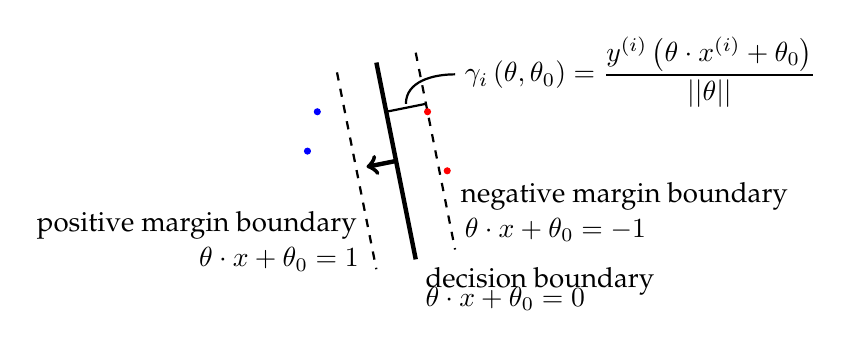
\begin{tikzpicture}[scale=0.5]
			\draw[thick,dashed] (0,5) -- (1,0);
			\draw[ultra thick,-] (1,5.25) -- (2,0.25);
			\draw[thick,dashed] (2,5.5) -- (3,0.5);
			\node[right] at (3,1) {$\theta\cdot x+\theta_0=-1$};
			\node[above right] at (2.9,1.25) {negative margin boundary};
			\node[above left] at (0.75,0.5) {positive margin boundary};
			\node[left] at (0.8,0.25) {$\theta\cdot x +\theta_0=1$};
			\draw [fill,red] (2.3,4) circle [radius=0.075];
			\draw [fill,red] (2.8,2.5) circle [radius=0.075];
			\draw[ultra thick, ->] (1.5,2.75) -- (0.75,2.6);
			\node[below right] at (2,0.3) {decision boundary};
			\node[below right] at (2,-0.2) {$\theta\cdot x+\theta_0=0$};
			\draw [fill, blue] (-0.5,4) circle [radius=0.075];
			\draw [fill, blue] (-0.75,3) circle [radius=0.075];
			\draw[thick, -] (1.25,4) -- (2.25,4.2);
			\draw[thick] (1.75,4.2) to [out=90,in=180] (3,4.95);
			\node[right] at (3,5) {$\gamma_i\left(\theta,\theta_0\right)=\dfrac{y^{(i)}\left(\theta\cdot x^{(i)}+\theta_0\right)}{||{\theta}||}$};
			\end{tikzpicture}
		\end{center}

		\begin{itemize}
			\item[] {\bf Distance from Decision to Margin} is $\dfrac{1}{\theta}$ after scaling (k = 1)
			\item[] {\bf Objective Function} $$J\left(\theta,\theta_0\right)=\frac{1}{n}\sum_{i=1}^{n}\left[\text{Loss}_h\left(y^{(i)}\left(\theta\cdot x^{(i)}+\theta_0\right)\right)+\frac{\lambda}{2}\lVert\theta\rVert^2\right]$$
	$\lambda$ is the regularization factor.
			\item [] {\bf Derivative}
				\begin{itemize}
					\item if Loss $>$ 0 $\Delta J = - y^{i} X^{(i)}$
					\item if Loss $=$ 0 $\Delta J = 0$
				\end{itemize}
		\end{itemize}

	\item[Recommender Systems]~
		$$Y_{n*m}$$ n users, m movies. Key is to borrow preferences from other users and measure how much a user is close to others
		\begin{itemize}
			\item[] {\bf $K$-Nearest Neighbor Method} Does not allow to identify hidden structure in the data
				$$\widehat{Y}_{ai}=\dfrac{\sum\limits_{b\in\text{KNN}(a)}\text{sim}(a,b)Y_{bi}}{\sum\limits_{b\in\text{KNN}(a)}\text{sim}(a,b)}$$
			\item[] {\bf Collaborative Filtering with Matrix Factorization}
				$$Y_{n*m} = U_{n*d} V_{d*m}^T$$
				$$J(X)=\sum_{(a,i)\in D}\frac{1}{2}\left(Y_{ai}-\left[UV^\intercal\right]_{ai}\right)^2+\frac{\lambda}{2}\left(\sum_{a,k}U_{ak}^2+\sum_{i,k}V_{ik}^2\right).$$
				To find the solution, we fix (initialize) $U$ (or $V$) and minimize the objective with respect to $V$ (or $U$). We plug-in the result back to the objective and minimize it with respect to $U$ (or $V$). We repeat this alternating process until there is no change in the objective function.
				\item For the case $k=1$. Then, $U_{a1}=u_a$ and $V_{i1}=v_i$. If we initialize $u_a$ to some values, then we have to optimize the function
				$$\sum_{(a,i)\in D}\frac{1}{2}\left(Y_{ai}-u_av_i\right)^2+\frac{\lambda}{2}\sum_{i}v_{i}^2.$$
		\end{itemize}
\end{description}

\section{Kernel}
Inner products between high dim vectors are cheap. Use kernel but not explicitly the high dim vector representation
$$K\left(x,x'\right)=\phi(x)\cdot\phi(x')$$
\begin{description}
	\item[Kernel Perceptron]
		$$\theta=\sum_{j=1}^{n}\alpha_jy^{(j)}\phi\left(x^{(j)}\right)$$
		$$\theta\cdot\phi\left(x^{(i)}\right)=\sum_{j=1}^{n}\alpha_jy^{(j)}\underbrace{\phi\left(x^{(j)}\right)\cdot\phi\left(x^{(i)}\right)}_{K\left(x^{(j)},x^{(i)}\right)}$$
		\begin{itemize}
			\item   For  {$t=1,\dots,T$}, {$i=1,\dots,n$}
			\item If {$y^{(i)}\sum\limits_{j=1}^{n}\alpha_jy^{(j)}K\left(x^{(j)},x^{(i)}\right)\leq0$}
						$$\alpha_j=\alpha_j+1$$
		\end{itemize}
	\item[Kernel Composition Rules]~
		\begin{enumerate}
			\item $K(x,x')=1$ is a kernel function.($\phi(x)=1$)
			\item Let $f:\mathbb{R}^d\rightarrow\mathbb{R}$ and $K(x,x')$ is a kernel. Then so is $\widetilde{K}(x,x')=f(x)K(x,x')f(x').$  ($\phi(x) = f(x)\phi(x)$)
			\item If $K_1(x,x')$ and $K_2(x,x')$ are kernels, then $K(x,x')=K_1(x,x')+K_2(x,x')$ is a kernel. $\phi(x) = [\phi_1(x), \phi_2(x)]^T$
			\item If $K_1(x,x')$ and $K_2(x,x')$ are kernels, then $K(x,x')=K_1(x,x')K_2(x,x')$ is a kernel.
		\end{enumerate}
	\item[Radial Basis Kernel]
		$$K(x, x') = e^{-\dfrac{1}{2}||x-x'||^2}$$
\end{description}




\section{Neural Network}
\begin{description}
	\item {\bf Motivation}: learn classifier and feature representation at the same time to improve performance. 
	\item {\bf Overcapacity}: Large models tend to be easier to learn because their units need to be adjusted so that they are, collectively sufficient to solve the task
	\item {\bf Backpropagation}~
		\begin{itemize}
			\item {\bf Model Setup}~
				$$Loss = C(a^L)$$
				$$a_j^l = f(\sum_k w_{jk}^l a_k^{l-1} + b_j^l)$$
				$$z_j^{l} = \sum_k w_{jk}^{l} a_k^{l-1} + b_j^l$$
					\begin{itemize}
						\item $b_j^l$ is the bias of the j-th neuron in the l-th layer
						\item $a_j^l$ is the activation of j-th neuron in the l-th layer
						\item $w_{jk}^l$ is the weight for the connection from the k-th neuron in the (l-1)-th layer to the j-th neuron in the l-th layer
					\end{itemize}
			\item {\bf Chain} define $\delta^l = \dfrac{\partial C}{\partial z_j^l}$
				$$\delta^{L} = \dfrac{\partial C}{\partial a_j^L}f'(z_j^L)$$
				$$\delta^l = \sum_k w_{kj}^{l+1}\delta_k^{l+1}f'(z_j^l)$$
				$$\dfrac{\partial C}{\partial w_{jk}^l} = a_k^{l-1} \delta_j^l$$
				$$\dfrac{\partial C}{\partial b_j^l} = \delta_j^l$$

		\end{itemize}
\end{description}

\section{Unsupervised Learning}
\begin{description}
	\item[Clustering: Input] ~
	\begin{itemize}[]
		\item Set of feature vectors $S_n=\left\{\left.x^{(i)}\right|i=1,\dots,n\right\}$
		\item The number of clusters $K$
	\end{itemize}
	\item[Clustering: Output] ~
	\begin{itemize}[]
		\item A partition of indices $\left\{1,\dots,n\right\}$ into $K$ sets, $C_1,\dots,C_K$
		\item {\it Representatives} in each of the $K$ partition sets, given as $z_1,\dots,z_K$
	\end{itemize}
	\item[Cost] We can calculate the total cost by summing the cost of each cluster:
	$$\text{Cost}\left(C_1,\dots,C_K\right)=\sum_{j=1}^{K}\text{Cost}\left(C_j\right)$$

	\item[Similarity Measure] ~
		\begin{itemize}
			\item We use the Euclidean distance between the elements of a cluster and its representative to calculate the cost for each cluster. Then, the total cost is
			$$\text{Cost}(C_1,...,C_K, z_1,...,z_K) = \sum_{j=1}^K \sum_{i \in C_j} || x^{(i)}-z_j||^2$$
			\item Cosine Distance: invariant to magnitude of the vectors
			$$dist(X^{(i)}, X^{(j)}) = \dfrac{X^{(i)} .  X^{(j)}}{||X^{(i)}|| *  ||X^{(i)}||}$$
		\end{itemize}

	\item[K-Mean Algorithm]~
		\begin{enumerate}
			\item Randomly select $z_1,\dots,z_K$.
			\item Iterate:
			\begin{enumerate}
				\item Given $z_1,\dots,z_K$, assign each data point $x^{(i)}$ to the closest $z_j$ so that
				$$\text{Cost}\left(z_1,\dots,z_K\right)=\sum_{i=1}^{n}\min\limits_{j=1,\dots,K}||x^{(i)}-z_j||^2.$$
				\item Given $C_1,\dots,C_K$, find the best representatives $z_1,\dots,z_K$, i.e., find $z_1,\dots,z_K$ such that
				$$z_j=\argmin\limits_{z}\sum_{i\in C_j}||{x^{(i)}-z}||^2=\dfrac{1}{\left|C_j\right|}\sum\limits_{i\in C_j}x^{(i)}.$$
			\end{enumerate}
			\begin{itemize}
				\item Local Solution (May run into troubles when initial rep are close to each other)
				\item Not robust to outliers
				\item Does not scale well with large dim: With increasing number of dims, a distance-based similarity measure converges to a constant value between any given examples
				\item {\bf Computational complexity}: O(ndK)
			\end{itemize}
		\end{enumerate}

	\item[K-Medoids Algorithm]~
		\begin{enumerate}
			\item Randomly select $\left\{z_1,\dots,z_K\right\}\subseteq\left\{x_1,\dots,x_n\right\}$.
			\item Iterate:
			\begin{enumerate}
				\item Given $z_1,\dots,z_K$, assign each $x^{(i)}$ to the closest $z_j$ so that
				$$\text{Cost}\left(z_1,\dots,z_K\right)=\sum_{i=1}^{n}\min\limits_{j=1,\dots,K}\text{dist}\left(x^{(i)},z_j\right)$$
				\item Given $C_j\in\left\{C_1,\dots,C_K\right\}$, find the best representative $z_j\in\left\{x_1,\dots,x_n\right\}$ such that
				$$\sum\limits_{x^{(i)}\in C_j}\text{dist}\left(x^{(i)},z_j\right)$$
				is minimal.
			\end{enumerate}
		\end{enumerate}
		\begin{itemize}
			\item {\bf Computational complexity}: $O(ndK) + O(n^2dK)$
		\end{itemize}

	\item[Generative Model]~
		\begin{itemize}
			\item {\bf Generative vs. Discriminative Models} {\it Generative models} work by explicitly modeling the probability distribution of each of the individual classes in the training data. {\it Discriminative models} learn explicit decision boundary between classes.
			\item[] {\bf Multinomial Generative Model}~
				$$\mathbb{P}\left(w|\theta\right)=\theta_w,\quad\theta_w\geq0,\sum_{w\in W}\theta_w=1.$$
					Then, the probability of generating the document $D$ is
					$$\mathbb{P}\left(D|\theta\right)=\prod_{i=1}^{n}\theta_{w_i}=\prod_{w\in W}\theta_w^{\,\text{count}(w)}.$$
					\item[Maximum Likelihood Estimate] 
					$$\widehat{\theta}_w=\dfrac{\text{count}(w)}{\sum\limits_{w'\in W}\text{count}(w')}.$$
					\item[] {\bf Prediction} Consider using a multinomial generative model $M$ for the task of binary classification consisting of two classes: $+$ (positive class) and $-$ (negative class).
					\begin{itemize}
						\item $\theta^+$: parameter for the positive class
						\item $\theta^-$: parameter for the negative class
					\end{itemize}
					Suppose that we classify a new document $D$ to belong to the positive class if and only if
					$$\log\dfrac{\mathbb{P}(D|\theta^+)}{\mathbb{P}(D|\theta^-)}\geq0.$$
					The generative classifier is equivalent to a linear classifier:
					$$\log\dfrac{\mathbb{P}(D|\theta^+)}{\mathbb{P}(D|\theta^-)}=\sum_{w\in W}\text{count}(w)\log\dfrac{\theta_w^+}{\theta_w^-}=\sum_{w\in W}\text{count}(w)\,\theta'_w.$$
					\item[] {\bf Baye} ~
					$$\mathbb{P}\left(y=+|D\right)=\dfrac{\mathbb{P}(D|\theta^+)\,\mathbb{P}(y=+)}{\mathbb{P}(D)}.$$
					$$\log\dfrac{\mathbb{P}\left(y=+|D\right)}{\mathbb{P}\left(y=-|D\right)}=\sum_{w\in W}\text{count}(w)\,\theta'_w+\theta'_0$$
	where $\theta'_w=\log\dfrac{\theta^+_w}{\theta^-_w}$ and $\theta'_0=\log\dfrac{\mathbb{P}(y=+)}{\mathbb{P}(y=-)}$.
	
					\item[] {\bf Generative Gaussian}~
						$X \in \mathbb{R}^d$ with mean $\mu \in \mathbb{R}^d$ and the same standard deviation $\sigma$ (uncorrelated)
						$$f_X\left(\mathbf{x}|\mu,\sigma^2\right)=\dfrac{1}{\left(2\pi\sigma^2\right)^{d/2}}\exp(-\dfrac{1}{2\sigma^2}||\mathbf{x}-\mu||^2).$$
					      $$\widehat{\mu}=\frac{1}{n}\sum_{i=1}^{n}\mathbf{x}^{(i)}$$
						$$\widehat{\sigma}^2=\frac{1}{nd}\sum_{i=1}^{n} ||\mathbf{x}^{(i)}-\mu||^2$$
					\end{itemize}
\end{description}

\subsection{EM Algorithm}
\begin{description}
	\item[Gaussian Mixture Models] 
	$$p(\mathbf{x}|\theta)=\sum_{j=1}^{K}p_j\mathcal{N}\left(\mathbf{x};\mu^{(j)},\sigma_j^2\mathbf{I}\right).$$
	For the training set
	$$S_n=\left\{\mathbf{x}^{(i)}, i=1,\dots,n\right\},$$
	the likelihood is
	$$\mathbb{P}\left(S_n|\theta\right)=\prod_{i=1}^{n}\sum_{j=1}^{K}p_j\mathcal{N}\left(\mathbf{x}^{(i)};\mu^{(j)},\sigma_j^2\mathbf{I}\right).$$
	\item[Observed Case] Consider the case of hard clustering, i.e., a point either belongs to a cluster or not. Let
	$$\delta(j|i)=
	\begin{cases}
		1,\quad&\mathbf{x}^{(i)}\text{ is assigned to }j\\
		0,&\text{otherwise}.
	\end{cases}$$
	Also, let $\widehat{n}_j=\sum\limits_{i=1}^{n}\delta(j|i)$ denote the number of points belonging to cluster $j$. Maximizing the likelihood gives
	\begin{align*}
		\widehat{p}_j&=\dfrac{\widehat{n}_j}{n}\\
		\widehat{\mu}^{(j)}&=\dfrac{1}{\widehat{n}_j}\sum_{i=1}^{n}\delta(j|i)\,\mathbf{x}^{(i)}\\
		\widehat{\sigma}^2_j&=\dfrac{1}{\widehat{n}_jd}\sum_{i=1}^{n}\delta(j|i)\,||\mathbf{x}^{(i)}-\mu^{(j)}||^2.
	\end{align*}
	\item[The EM Algorithm] Instead of hard clustering, the data can actually be generated from different clusters with different probabilities. We have soft clustering. We can maximize the likelihood through the EM algorithm.
	\begin{enumerate}
		\item[] Randomly initialize $\theta$: $\mu^{(1)},\dots,\mu^{(K)},\sigma^2_1,\dots,\sigma^2_K,p_1,\dots,p_K.$
		\item {\bf E-step:}
		$$p(j|i)=\dfrac{p_j\mathcal{N}\left(\mathbf{x}^{(i)};\mu^{(j)},\sigma^2_j\mathbf{I}\right)}{p\left(\mathbf{x}|\theta\right)}$$
		where $p(\mathbf{x}|\theta)=\sum\limits_{j=1}^{K}p_j\mathcal{N}\left(\mathbf{x}^{(i)};\mu^{(j)},\sigma^2_j\mathbf{I}\right)$
		\item {\bf M-step:}
		\begin{align*}
			\widehat{n}_j&=\sum_{i=1}^{n}p(j|i)\\
			\widehat{p}_j&=\dfrac{\widehat{n}_j}{n}\\
			\widehat{\mu}^{(j)}&=\dfrac{1}{\widehat{n}_j}\sum_{i=1}^{n}p(j|i)\,\mathbf{x}^{(i)}\\
			\widehat{\sigma}^2_j&=\dfrac{1}{\widehat{n}_jd}\sum_{i=1}^{n}p(j|i)||\mathbf{x}^{(i)}-\mu^{(j)}||^2.
		\end{align*}
	\end{enumerate}
\end{description}

\section{Reinforcement Learning}
Goal: Learn a good policy with none or limited supervision
\begin{description}
	\item[MDP]~
		\begin{itemize}
			\item {\bf Transition} $T(s, a, s') = \mathbb{P}(s'|s, a)$
			\item {\bf Reward} $R(s, a, s')$. The reward of starting at s, taking action a and ending up at $s'$ 
		\end{itemize}
	\item[Utility]~
		\begin{itemize}
			\item {\bf Infinite Utility} $U[s_0,s_1,\dots]=\sum_{k=0}^{\infty}\gamma^kR(s_k).$
			\item An finite step utility function can depend on steps left (I.E. very few steps left may lead to risk taking behavior)
			\item Inifnite discounted utility make the utility depend on current step only
			\item Infinite discunted utility converge to $\dfrac{R_{min}}{1-\gamma}$
			\item {\bf Policy} $\pi(s)$ that assign an action $\pi$ to the state s
			\item {\bf Optimal Policy} $\pi_s^{\star} = argmax_{a_s}\mathbb{E}[U(a_s)]$
		\end{itemize}

	\item[Bellman Equations]~
		\begin{itemize}
			\item {\bf Value Function} $V(s)$ expected reward starting from state s and acting optimally ever since
				$$V(s) = \max_{a}Q(s, a) = Q(s,\pi^{\star}(s))$$
			\item {\bf Q Function} $Q(s, a)$ expected reward strating at s, acting with acting a and then acting optimally aftewrwards
				$$Q(s, a)=\sum_{s'}T(s,a,s')(R(s,a,s')+\gamma V(s'))$$
			\item{\bf Value Iteration} $V(s) = \max_{a}\sum_{s'}T(s,a,s')(R(s,a,s')+\gamma V(s')$
				$$V_{k+1}(s) = \max_{a}\sum_{s'}T(s,a,s')[R(s,a,s')+\gamma V_k(s')]$$
			\item For the iterations, can plug in the final value to the rhs and solve for value
			\item {\bf Q-value Iteration} 
				$$Q_{k+1}(s, a)=\sum_{s'}T(s,a,s')[R(s,a,s')+\gamma \max_{a'}Q_{k}(s', a')]$$
			\item Value Iteration will finally converge as long as $\gamma <1$ (speed for one iterationL $O(|S|^2 |A|)$)
				$$V(s) - V_k(s) = \gamma (V(s) - v_{k-1}(s))$$
		\end{itemize}
		\item[Q-Value Iteration for RL] ~
			\begin{enumerate}
				\item Initialization: $Q(s,a)=0\;\forall s,a$
				\item Iterate until convergence:
				\begin{enumerate}
					\item Collect sample: $s,a,s',R(s,a,s')$
					\item Update:
					\begin{align*}
						Q_{i+1}(s,a)&\leftarrow\,\alpha\left[R(s,a,s')+\gamma\max\limits_{a'}Q_i(s',a')\right]+(1-\alpha)\,Q_i(s,a)\\
						&=Q_i(s,a)+\alpha\left[R(s,a,s')+\gamma\max\limits_{a'}Q_i(s',a')-Q_i(s,a)\right]
					\end{align*}
				\end{enumerate}
			\end{enumerate}
		\item[Exploration]~
			\begin{itemize}
				\item Exploitation (Optimal) $1-\epsilon$ 
				\item Exploitation (Random) $\epsilon$ should decay as get data
			\end{itemize}
		\item[NLP]~
			\begin{itemize}
				\item Difficulty arises from ambiguity intrinsic in natural languages
				\item {\bf Approaches}
					\begin{enumerate}
						\item Symbolic: Structured rules. Encode all required info into an elaborate knowledge representation
						\item Statistical: Infer language properties from large language samples.
					\end{enumerate}
				\item {\bf Word Embedding}
					\begin{enumerate}
						\item cosine similarity between words are used for a much sparse encoding
						\item Bag of words approach sums up all the word embeddings to encode hence does not capture sequence
					\end{enumerate}
			\end{itemize}
					
\end{description}

\section{Recurrent Network}
\begin{description}
	\item {\bf Motivation}: Model the sequence. How history is mapped to a feature vector (encoding) is alos part of the learning process
	\item {Difference with FF}
		\begin{itemize}
			\item Inputs received at each layer. 
			\item Layer number depend on lenght of sentence
			\item parameters of each layer are shared
		\end{itemize}
	\item {\bf Basic RNN}
		$$s_t  = tanh(W^{s,s}s_{t-1} + W^{s,x}x_t)$$
		\begin{itemize}
			\item Gradient can vanish or explode since the sequences are long and we apply transformation repeatedly. Can resolve by introducing gate
		\end{itemize}
	\item {\bf Simple Gated RNN}
		\begin{align*}
			g_t&=\text{sigmoid}\left(W^{g,s}s_{t-1}+W^{g,x}x_t\right)\\
			s_t&=\left(1-g_t\right)\odot s_{t-1}+g_t\odot\tanh(W^{s,s}s_{t-1}+W^{s,x}x_t)
		\end{align*}
	\item {\bf LSTM}
		\begin{alignat*}{2}
			f_t&=\text{sigmoid}\left(W^{f,h}h_{t-1}+W^{f,x}x_t\right)\quad&&{\text{forget gate}}\\
			i_t&=\text{sigmoid}\left(W^{i,h}h_{t-1}+W^{i,x}x_t\right) &&{\text{input gate}}\\
			o_t&=\text{sigmoid}\left(W^{o,h}h_{t-1}+W^{o,x}x_t\right) &&{\text{output gate}}\\
			c_t&=f_t\odot c_{t-1}+i_t\odot\tanh(W^{c,h}h_{t-1}+W^{c,x}x_t) \quad&&{\text{memory cell}}\\
			h_t&=o_t\odot\tanh(c_t)&&{\text{visible state}}
		\end{alignat*}	
	\item {\bf Markov Model (First-Order)}
		\begin{itemize}
			\item Consist of an UNK symbol for any word, <beg>, <end>
			\item {\bf Bigram Model} $\prod_{i=1} \mathbb{P}(w_i|w_{i-1})$
			\item ML estimation: $\widehat{\mathbb{P}}(w'|w) = \dfrac{count(w', w)}{\sum_{w_i} count(w, w_i)}$
		\end{itemize}
	\item {\bf Markov Model to FNN}
		$$z_k = \sum_j x_j W_{jk} + W_{0,k},   k \in \mathbb{R}$$
		$$P_k = P(w_i=k|w_{i-1}) = \dfrac{e^{z_k}}{\sum_{j=1}^K e^{z_j}}$$
		\begin{itemize}
			\item Advantages: Fewer number of parameters, easily to control complexity by introducing hidden layers
			\item Triagram: $2K^2+K$ vs $K^3$
		\end{itemize}
	\item {\bf Markove Model to RNN} At each step
		$$s_t = tanh(W^{s,s}s_{t-1} + W^{s,w}x_t)$$
		$$p_t = softmax(W^0 s_t)$$ or more complext like LSTM
		$$p_t = softmax(W^0 h_t)$$
 
\end{description}

\section{CNN}
Goal: Extend local learning globally
\begin{description}
	\item{\bf convolution} stride: layer l is obtained by slid (convolute) across the image at layer l-1 with a small kernel
		$$\left(f*g\right)(t)\equiv\int_{-\infty}^{+\infty}f(\tau)g(t-\tau)d\tau.$$
		$$\left(f*g\right)[n]\equiv\sum_{m=-\infty}^{m=+\infty}f[m]g[n-m].$$
	\item{\bf Pool}: Further dim reduction. Can help to identify whether a feature is there withou knowing where it is 
		\begin{itemize}
			\item Induce translation invariance at cost of spatial resolution
			\item Stried help to reduce the size 
		\end{itemize}
\end{description}






\section{python}
\begin{description}
	\item[Distribution] ~
		\begin{itemize}
			\item scipy.stats.binom(n=n, p=p)
			\item scipy.stats.poisson(mu=mu)
			\item scipy.stats.norm()
			\item scipy.stats.chi(df=df)
		\end{itemize}
	\item[Distribution Function]~
		\begin{itemize}
			\item $1 - \alpha$ = rv.cdf($q_{\alpha}$) 
			\item $q_{\alpha}$ = rv.ppf($1 - \alpha$)
			\item $\alpha$ = rv.sf($q_{\alpha}$)
			\item $q_{\alpha}$ = rv.isf($\alpha$)
		\end{itemize}
	\item[Hypothesis Test]~
		\begin{itemize}
			\item {\bf Fisher exact test} scipy.stats.fisher$\_$exact(np.array([[$x_{test}$, $x_{cont}$], [$n_{test}$, $n_{cont}$] ]), 'less') with less in alternative hypothesis
			\item {\bf One sample t test} scipy.stats.ttest$\_$1samp(array, popmean=$H_0$, alternative='greater')
			\item If nul rejected by Bonferroni, then it is also rejected by HB. Power of HB is greater than or equal to that of Bonferroni
			\item If nul rejected by HB then it is always rejected by BH
			\item Restriction on FWER is more strict
			\item {\bf Multi Test Correction} statsmodels.stats.multitest.multipletests(pvals, alpha=0.05, method='holm')
			\item statsmodels.api.qqplot(x,line='s')		
			\item {\bf Likelihood}: scipy.stats.poisson.pmf(gamma$\_$data['count'], gamma$\_$data['seconds']*lamb).prod(axis=0)
			\item Lambda$\_$observed = -2*np.log(likelihood$\_$H0(lambda$\_$hat$\_$H0)/likelihood$\_$H1(lambdas$\_$hat$\_$H1))	
			\item scipy.stats.kstest
	\end{itemize}
\end{description}



\end{multicols*}
\end{document}